% introduzindo a jogos, por que é um mercado que está tao em alta
A indústria de jogos digitais cresce cada vez mais, de acordo com \space\citeonline{quanto_games_vao_movimentar}, essa indústria tende a ultrapassar em 2023, os US\$ 200 bilhões (aproximadamente, R\$ 1 trilhão). Novos jogos são produzidos e publicados diariamente, e somente na plataforma digital Steam, foram 10.963 novos títulos em 2022\space
\cite{numero_de_jogos_publicados_na_steam}.

% aqui a gente aproveita que falou de jogos para introduzir MAPAS que é o 'tema' do tcc
No cenário de jogos, os mapas desempenham um papel fundamental, fornecendo orientação aos jogadores e criando a sensação de escala em uma área. Por exemplo o jogo de aventura pirata chamado Sea of Thieves, os mapas revelam locais de interesse, como tesouros escondidos, missões e áreas perigosas. Ajudam os jogadores a planejar suas estratégias, explorar o mundo virtual e tomar decisões com base em informações espaciais. Portanto os mapas enriquecem a experiência geral do jogo, mas cria-los pode ser um desafio, especialmente levando em consideração o orçamento disponível. Pois demandaria muitos recursos criar vários mapas diferentes com intuito de entretenimento do jogador, em jogos como Minecraft um elemento importante é a forma procedural no qual se cria os mundos, com ilhas contendo biomas, cavernas, vilas, dentre outros recursos. Com essa diversidade de características pode-se evitar o tédio de sempre jogar no mesmo mapa \cite{video-game-maps, lecafedugeek}.

% \begin{figure}[H]
% 	\caption{Mapa de tesouro do jogo Sea of Thieves}
% 	\centering % para centralizarmos a figura
% 	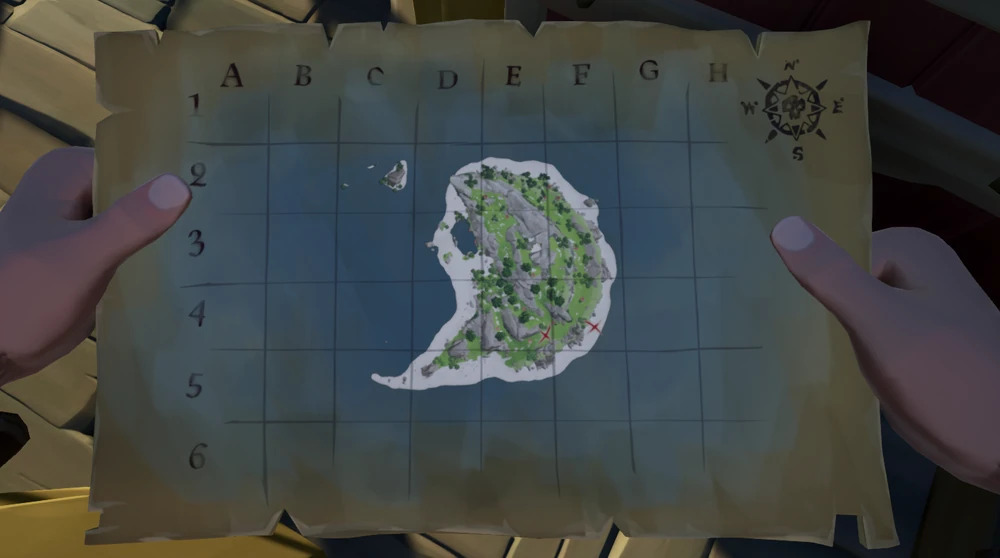
\includegraphics[width=10cm]{figures/Treasure_Map.jpg} % leia abaixo
% 	\legend{Fonte: \citeonline{seaofthieves}}
% 	\label{fig:treasureMap}
% \end{figure}

% aqui a gente faz um adendo e a demanda de jogos tende a crescer, então da a entender que voce tem que produzir cada vez mais
% e tambem fala o quanto custa para produzir um jogo
% Ademais, o mercado de jogos no Brasil teve um aumento de 2,5\% em 2022, como apontado por uma pesquisa sobre o crescimento da demanda \space \cite{pesquisa_games_brasil}. O custo de produção de jogos varia bastante, dependendo do tamanho e da complexidade do projeto, \emph{e.g.}, a empresa Rockstar Games revelou que o jogo \textit{Grand Theft Auto V} custou cerca de 265 milhões de dólares para ser desenvolvido e comercializado \space \cite{gta_quanto_custou}.

%solucao para o problema 
% Apesar do rápido crescimento da indústria, existe uma carência de ferramentas que possam auxiliar os designers e artistas durante o processo de produção de jogos, o que acaba tornando-o demorado e, consequentemente, mais caro.  Segundo o livro "Procedural Content Generation in Games" \cite{procedural_centent_book}, uma abordagem eficiente para reduzir os custos de produção de um jogo é utilizar a geração procedural de conteúdo. Essa técnica permite maximizar o desenvolvimento de um jogo, envolvendo o uso de um software de computador capaz de criar conteúdo de jogos automaticamente. Esse software possibilita a geração automatizada de mapas, otimizando o processo de desenvolvimento.

% No entanto, a criação de mapas usando esse método ainda encontram dificuldades, sendo elas, variedade e autenticidade \cite{geracao_procedural_jogos_2d}.
% aqui adicionar uma explicação do porque é um desafio a geração procedeural de conteudo 

% introduz a relação de ia para personalização dentro de métodos procedurais em jogos
De acordo com \citeonline{jogo_procedural} é muito comum usar técnicas procedurais combinado com inteligência artificial para melhorar ou personalizar a experiência do jogador. Por exemplo, o jogo RimWorld é um simulador de colônia que gera um planeta de forma procedural e utiliza uma IA para narrar a história, abrangendo psicologia, ecologia, combate e diplomacia, dentre outros. Logo, essa combinação entre IA e a geração procedural cria uma jogabilidade única ao jogador.

% A aplicação da IA em jogos não se limita apenas à jogabilidade. Ela também é usada em áreas como animação de personagens, reconhecimento de fala e expressões faciais, tradução automática de idiomas nos diálogos do jogo e muito mais. A IA está impulsionando a inovação e a evolução dos jogos, proporcionando experiências cada vez mais envolventes e cativantes para os jogadores \cite{exameNvidia, omniverseace}.

% introduz o ramo de segmentação geral que será explicado mais para frente
Em IA, um ramo que está em ascensão é o de segmentação de imagem com redes neurais convolucionais, onde é possível classificar os pixeis de uma imagem, criar máscaras  para destacar cada objeto\footnote{Todas classes que são contáveis como pessoas, carros, etc.} detectado. As suas aplicações são diversas como por exemplo, carros ou drones autônomos, sistemas de vigilância, sistemas militares inteligentes, entre outros. Nessas aplicações é possível observar que é preciso ter um foco em identificar e segmentar seres humanos, por exemplo, em carros autônomos é primordial essa tarefa para o carro tomar a decisão de frear quando estiver muito perto de bater. Logo, se torna um tópico relevante dentro de visão computacional, no qual pode ter diversas aplicações no mundo real \cite{kirillov2019panoptic, dp_semantic_segmantation}.

Por conseguinte, a combinação entre inteligência artificial e geração procedural de mapas pode abrir novas possibilidades de personalização nos jogos. Imagine um jogo em que, a partir da segmentação de imagens por meio de redes neurais convolucionais, os jogadores possam criar mapas únicos e personalizados para suas aventuras. Com uma foto, o modelo treinado segmentaria a imagem para selecionar um contorno reconhecido, e a partir dele se criar um mapa de maneira procedural contendo biomas no mesmo formato escolhido. 

No contexto da geração procedural de mapas, explorar a relação entre IA e personalização de jogos contribuirá para o avanço dessas áreas de pesquisa, proporcionando aos jogadores experiências mais ricas e variadas.

% Adicionar uma parte explicando a parte de visão computacional e porque o tema da nossa Ia é identificação de pessoas 

% Dito isso, nosso projeto tem a ideia de fornecer recursos baseados em matemática aplicada dentro de ciência da computação que proporcione uma funcionalidade de escolher o contorno do mapa no qual irá jogar através de imagens. Abordaremos a arquitetura de redes neurais convolucionais, que é muito utilizada para trabalhar com imagens. Mais especificamente, abordaremos uma arquitetura derivada da arquitetura mencionada anteriormente, específica para segmentação de imagens, o que possibilita classificar contornos em imagens.

\section{Objetivos}

O objetivo principal deste trabalho é desenvolver uma ferramenta que ofereça uma alternativa para a geração procedural de mapas de ilhas, utilizando o diagrama de Voronoi para a criar biomas. Além disso, pretende-se combinar segmentação com redes neurais convolucionais para permitir a personalização desses mapas. Essa ferramenta terá a capacidade de reconhecer os contornos\footnote{Os contornos reconhecidos são os classificados no conjunto de dados, logo o resultado terá uma detecção abrangente dentro do escopo de classes obtidas} de uma imagem, e gerar um mapa que preserva fielmente o contorno escolhido.

Adicionalmente, os seguintes objetivos específicos serão abordados:

\begin{itemize}
	\item Selecionar e analisar conjuntos de dados contendo classes relevantes, como pessoas, carros, entre outros, para treinar um modelo de rede neural convolucional específico para segmentação de imagens.
	\item Avaliar o desempenho geral do modelo usando a métrica de avaliação específica para o nicho de segmentação selecionado.
	\item Testar algoritmos de gerar ruídos para criar o mapa.
	\item Aplicar um algoritmo para reconhecer a imagem com o contorno selecionado e gerar como resultado a imagem do mapa gerado.
\end{itemize}

% Outro cenário que está crescendo muito nos últimos anos é o da inteligência artificial, afirma \citeonline{Valente_2020} que no Brasil mais que dobrou o número contratações de desenvolvedores da área de 2015 até 2020. De acordo com \apud{johnson2023}{briggs2023} um relatório recente relata que 300 milhões de empregos podem ser afetados pela IA \emph{i.e.} 18\% ofício global pode ser automatizado. Outrossim \citeonline{europarl2020} diz que o tópico de inteligência artificial é uma prioridade para União Europeia por ser considerada primordial para transformação digital da sociedade.  Do mesmo modo, Bill Gates, um dos fundadores da Microsoft — uma das maiores empresas de tecnologia —, diz que "o desenvolvimento da inteligência artificial (IA) é o avanço tecnológico mais importante em décadas"\space
% \cite{inteligencia_artificial_e_avanco_bbc}.